% !TEX program = xelatex
% Preview scope: Abstract, Introduction, System Model, Problem Formulation.
% Remaining section and subsection headings are deliberately empty.
\renewcommand{\rmdefault}{ptm}
\RequirePackage[T1]{fontenc}
\documentclass[conference]{IEEEtran}
\IEEEoverridecommandlockouts
\usepackage{mathptmx}
\usepackage{amsmath,amssymb,bm}
\usepackage{graphicx}
\usepackage{xcolor}
\usepackage[hidelinks]{hyperref}
\usepackage[capitalize,nameinlink,noabbrev]{cleveref}
\usepackage{microtype}
\newcommand{\UE}{\mathrm{UE}}
\newcommand{\BS}{\mathrm{BS}}
\newcommand{\EH}{\mathrm{EH}}
\newcommand{\DL}{\mathrm{DL}}
\newcommand{\RF}{\mathrm{RF}}
\newcommand{\fly}{\mathrm{fly}}
\newcommand{\hov}{\mathrm{hov}}
\newcommand{\tot}{\mathrm{tot}}
\newcommand{\setT}{\mathcal{T}_{\mathrm{s}}}
\newcommand{\setN}{\mathcal{N}}
\newcommand{\setM}{\mathcal{M}}
\newcommand{\norm}[1]{\left\lVert #1\right\rVert}
\interdisplaylinepenalty=2500
\pagestyle{plain}
\raggedbottom
\begin{document}
\title{Joint UAV Trajectory, NOMA Power Allocation and BS Deployment for Energy-Efficient SWIPT-Enabled Communications}
\author{Hoang Cao Minh, Ninh Thi Thanh Tam, Nguyen Minh Quan, and Trinh Van Chien
\thanks{Ninh Thi Thanh Tam is with the Faculty of Information and Communication Technology, National Academy of Education Management, Vietnam, and the School of Information and Communications Technology, Hanoi University of Science and Technology, Hanoi 100000, Vietnam (email: tam.ntt250098D@sis.hust.edu.vn).}
\thanks{Hoang Cao Minh, Nguyen Minh Quan, and Trinh Van Chien are with the School of Information and Communications Technology, Hanoi University of Science and Technology, Hanoi 100000, Vietnam (email: minh.hc2416559@sis.hust.edu.vn; quannm@soict.hust.edu.vn; chientv@soict.hust.edu.vn).}}
\maketitle
\thispagestyle{plain}

% SECTION-WRITING OBJECTIVE: State the design task immediately; define each
% quantity before use; explain each constraint beside its mathematical form.
% OUTLINE: Task and contributions -> geometry and timing -> channels -> EH
% -> NOMA payload -> energy -> variables/objective -> six constraint groups.
% CLAIM-EVIDENCE: Energy and payload definitions: V10 evaluator/model files,
% supported. PSO/IPSO mechanism: optimizer files, supported. Performance gains:
% no claim made; experimental section intentionally remains empty.
% SELF-REVIEW: Same physics and source scope as the first preview. No invented
% experimental result, global-optimality claim, or normalized alpha floor.

\begin{abstract}
This paper studies the joint design of UAV trajectory, NOMA power allocation, and base-station deployment to maximize downlink energy efficiency. A rotary-wing UAV harvests RF energy from multiple base stations and uses it to transmit data to ground users. The UAV flies at a fixed altitude and serves users while hovering at selected waypoints. Energy efficiency is defined as the total delivered bits divided by the UAV energy used for cruising, hovering, and RF transmission. The design must satisfy each user's mission data requirement, minimum service in every slot, an energy budget, and geometric constraints. We formulate the resulting nonconvex problem and consider particle swarm optimization and an improved variant with adaptive mutation to search for feasible solutions. The formulation captures the trade-off between better communication channels and the additional propulsion energy required to reach favorable service locations.
\end{abstract}
\begin{IEEEkeywords}
UAV communications, energy efficiency, SWIPT, NOMA, trajectory optimization, base-station deployment.
\end{IEEEkeywords}

\section{Introduction}
\label{sec:introduction}
We consider a UAV-assisted network in which ground base stations (BSs) supply RF energy to a UAV, and the UAV serves ground users through downlink non-orthogonal multiple access (NOMA). The objective is to deliver more data per joule of UAV energy while meeting each user's service requirements. Three decisions are coupled: where the UAV serves users, how its transmit power is shared among them, and where the BSs are deployed.

The coupling follows directly from the signal and energy paths. Moving the UAV changes both the BS-to-UAV energy supply and the UAV-to-user channels. Moving a BS changes the energy available for downlink transmission along the route. A trajectory detour may improve these channels, but it also increases propulsion energy. The design must therefore account for data delivery and flight energy together. Because users share the downlink through NOMA, their power allocation must also satisfy individual data requirements.

Related studies address different parts of this design. \href{https://arxiv.org/abs/1804.02238}{Zeng, Xu, and Zhang (2018)} optimize rotary-wing UAV energy consumption under individual throughput requirements.\footnote{Y. Zeng, J. Xu, and R. Zhang, \emph{Energy Minimization for Wireless Communication with Rotary-Wing UAV}, arXiv:1804.02238, 2018. \url{https://arxiv.org/abs/1804.02238}.} \href{https://doi.org/10.1109/VTC2024-Fall63153.2024.10758018}{Baduge, Perera, and Jayakody (2024)} use particle swarm optimization (PSO) for a minimum-rate objective in a SWIPT-enabled UAV-assisted NOMA network.\footnote{D. P. P. R. Baduge, T. D. P. Perera, and D. N. K. Jayakody, \emph{Flight to Efficiency: Trajectory Optimization in SWIPT-Enabled UAV-Assisted NOMA for Future Wireless Networks}, IEEE VTC2024-Fall, 2024, doi: 10.1109/VTC2024-Fall63153.2024.10758018.} \href{https://doi.org/10.3390/drones10040238}{Zhang et al. (2026)} jointly design UAV trajectory and power control for NOMA-enabled backscatter data collection.\footnote{T. Zhang, M. Gu, D. Mishra, J. Yuan, and A. Seneviratne, \emph{Trajectory and Power Control for Sustainable UAV-Assisted NOMA-Enabled Backscattering IoT}, Drones, vol. 10, no. 4, article 238, 2026, doi: 10.3390/drones10040238.} We use the multirotor propulsion expression in the latter study and explicitly include the energy spent hovering during communication service.

Our formulation combines horizontal UAV trajectory design, NOMA power allocation, and static BS deployment in a mission-level bits-per-joule objective. The UAV altitude, cruise speed, service duration, and SWIPT parameters are fixed. Both the total data delivered to each user and its data delivered in every service slot are constrained. The main contributions are:
\begin{itemize}
\item An energy-efficiency formulation that includes cruise, hover, and RF energy in a single UAV energy budget.
\item A joint design of UAV waypoints, NOMA power shares, and BS positions under geometric and user-service constraints.
\item A PSO-based solution framework, including an improved variant with adaptive mutation, for comparing fixed-BS and joint-deployment designs.
\end{itemize}

\section{System Model}
\label{sec:system_model}
\subsection{Network Geometry and Service Protocol}
The network contains one rotary-wing UAV, $M$ BSs, and $N$ ground users. Define $\setM=\{1,\ldots,M\}$ and $\setN=\{1,\ldots,N\}$. User $n$ is fixed at $\bm u_n=[x_n^{\UE},y_n^{\UE},0]^T$. BS $m$ is at $\bm b_m=[x_m^{\BS},y_m^{\BS},z_m^{\BS}]^T$. Its height $z_m^{\BS}$ is fixed, whereas its horizontal position $\bm s_m=[x_m^{\BS},y_m^{\BS}]^T$ is selected within a prescribed rectangle $\mathcal B_m$. BS positions remain unchanged during the mission.

The UAV follows $T$ waypoints at a fixed altitude $H$:
\begin{equation}
\bm q_t=[x_t,y_t,H]^T,\qquad t=1,\ldots,T.
\label{eq:waypoints}
\end{equation}
The initial and final waypoints are prescribed. Service takes place at waypoints $1,\ldots,T-1$, indexed by $\setT=\{1,\ldots,T-1\}$. At each service waypoint, the UAV first hovers to receive BS signals and harvest energy, then transmits data to the users, and finally flies to the next waypoint. The final waypoint is an arrival point with no additional service interval. \Cref{fig:1SystemModel} illustrates this protocol.

\begin{figure*}[t]
\centering
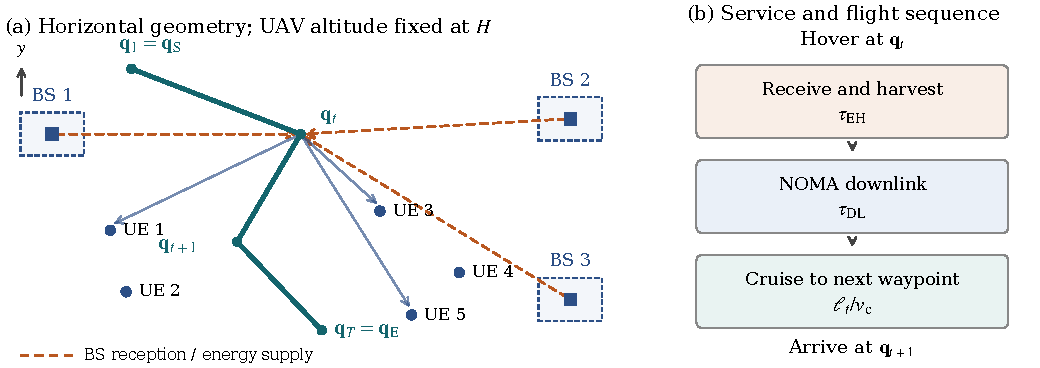
\includegraphics[width=\textwidth]{Images/system_model.pdf}
\caption{Network and service protocol. BS positions are selected within the dashed deployment regions. At each service waypoint, the UAV receives BS signals, harvests energy, and then transmits to users through downlink NOMA before flying to the next waypoint. The geometry is illustrative.}
\label{fig:1SystemModel}
\end{figure*}

Each hover interval has a fixed duration $\tau_{\hov}$, divided into
\begin{equation}
\tau_{\EH}=\lambda\tau_{\hov},\qquad
\tau_{\DL}=(1-\lambda)\tau_{\hov},\quad 0<\lambda<1,
\label{eq:phase_times}
\end{equation}
where $\tau_{\EH}$ and $\tau_{\DL}$ are the reception/harvesting and downlink durations. At cruise speed $v_{\mathrm c}$, segment $t$ has distance and flight time
\begin{equation}
\ell_t=\norm{\bm q_{t+1}-\bm q_t},\qquad
\tau_t^{\fly}=\frac{\ell_t}{v_{\mathrm c}}.
\label{eq:flight_time}
\end{equation}
The mission duration is $\sum_{t\in\setT}\tau_t^{\fly}+(T-1)\tau_{\hov}$. All segments, including the one entering the final waypoint, are counted. Data transmission occurs only during hovering.

\subsection{Channel Model}
\label{subsec:channel_assumptions}
For a user or BS at $\bm a_i=[a_{i,x},a_{i,y},a_{i,z}]^T$, define
\begin{align}
d_{t,i}&=\sqrt{(x_t-a_{i,x})^2+(y_t-a_{i,y})^2},\nonumber\\
r_{t,i}&=\sqrt{d_{t,i}^2+(H-a_{i,z})^2},\nonumber\\
\theta_{t,i}&=\operatorname{atan2}(|H-a_{i,z}|,d_{t,i}),
\label{eq:distances}
\end{align}
where $r_{t,i}>0$ is the link distance and $\theta_{t,i}\in[0,\pi/2]$ is the elevation magnitude. The large-scale power gain is
\begin{equation}
\beta_{t,i}=\beta_0\left(\frac{r_{t,i}}{r_0}\right)^{-\nu},
\qquad r_0=1\ \mathrm m,
\label{eq:path_loss}
\end{equation}
with reference gain $\beta_0$ and path loss exponent $\nu$. The Rician fading coefficient is
\begin{equation}
g_{t,i}=\sqrt{\frac{K_{t,i}}{K_{t,i}+1}}
+\sqrt{\frac{1}{K_{t,i}+1}}\,\widetilde g_i,
\label{eq:rician_fading}
\end{equation}
where $\widetilde g_i\sim\mathcal{CN}(0,1)$ and
\begin{equation}
K_{t,i}=K_{\min}\exp\!\left[
\frac{2\theta_{t,i}}{\pi}\ln\!\left(\frac{K_{\max}}{K_{\min}}\right)\right].
\label{eq:rician_k}
\end{equation}
The $K$-factor endpoints are in linear scale. One scattering sample is drawn for each physical link and held fixed across the mission and candidate designs. Channel changes within a scenario therefore follow from geometry.

The UAV-to-user and BS-to-UAV channels are
\begin{equation}
h_{t,n}=\sqrt{\beta_{t,n}^{\UE}}\,g_{t,n}^{\UE},\qquad
k_{t,m}=\sqrt{\beta_{t,m}^{\BS}}\,g_{t,m}^{\BS}.
\label{eq:channels}
\end{equation}
Locations and the channel realization are assumed known for offline design. Separate shadowing and inter-cell downlink interference are omitted.

\subsection{Energy Harvesting and RF Transmit Power}
Each BS transmits at a fixed power $P^{\BS}$. For independent BS signals, the received RF power and harvested energy are
\begin{align}
P_t^{\mathrm{rec}}&=P^{\BS}\sum_{m\in\setM}|k_{t,m}|^2,\label{eq:received_power}\\
E_t^{\EH}&=\eta\varphi P_t^{\mathrm{rec}}\tau_{\EH},
\label{eq:harvested_energy}
\end{align}
where $\varphi$ is the received-power fraction assigned to harvesting and $\eta$ is the conversion efficiency. Both are fixed in $[0,1]$. All harvested energy is used for RF transmission in the following downlink phase of the same service slot:
\begin{equation}
P_t=\frac{E_t^{\EH}}{\tau_{\DL}}
=\eta\varphi P^{\BS}\frac{\tau_{\EH}}{\tau_{\DL}}
\sum_{m\in\setM}|k_{t,m}|^2.
\label{eq:uav_power}
\end{equation}
The RF transmit power $P_t$ is thus determined by the geometry and SWIPT settings. The NOMA variables only divide this available power among users.

The information branch is assumed to supply enough data for downlink service. BS-to-UAV decoding rates and two-hop data causality are not modeled. Harvesting is linear, with ideal use of the harvested energy; storage losses, harvesting saturation, RF amplifier losses, and circuit loads are omitted. The onboard battery supplies propulsion.

\subsection{Downlink NOMA and Delivered Data}
Let $\pi_t$ sort users from weakest to strongest channel:
\begin{equation}
|h_{t,\pi_t(1)}|^2\le\cdots\le|h_{t,\pi_t(N)}|^2.
\label{eq:sic_order}
\end{equation}
Write $[u]=\pi_t(u)$ for rank $u$ in slot $t$. User $n$ receives power share $\alpha_{t,n}$, with nonnegative shares summing to one. A weaker channel is assigned at least as large a share. With superposition coding and ideal successive interference cancellation (SIC), the SINR and rate are
\begin{align}
\gamma_{t,[u]}&=
\frac{P_t\alpha_{t,[u]}|h_{t,[u]}|^2}
{\sigma^2+P_t|h_{t,[u]}|^2\sum_{j=u+1}^{N}\alpha_{t,[j]}},
\label{eq:sinr}\\
R_{t,n}&=B\log_2(1+\gamma_{t,n}),
\label{eq:rate}
\end{align}
where $B$ is the bandwidth, $N_0$ is the noise power spectral density, and $\sigma^2=N_0B$ is the common receiver noise power. Weaker-user messages are canceled; stronger-user messages remain as interference. The interference sum is zero for the strongest user.

The data delivered to physical user $n$ in slot $t$, its mission total, and the aggregate downlink payload are
\begin{align}
D_{t,n}&=\tau_{\DL}R_{t,n},\label{eq:slot_bits}\\
D_n&=\sum_{t\in\setT}D_{t,n},\qquad
D_{\tot}=\sum_{n\in\setN}D_n.
\label{eq:total_bits}
\end{align}
All three quantities are measured in bits. User requirements follow the physical user identity, even when its channel rank changes.

\subsection{UAV Energy Consumption}
The propulsion model has blade-profile, induced, and parasite components:
\begin{equation}
P_{\mathrm{prop}}(v)=P_{\mathrm{pro}}(v)
+P_{\mathrm{ind}}(v)+P_{\mathrm{par}}(v).
\label{eq:propulsion}
\end{equation}
Following the multirotor model of Zhang et al. (2026), the thrust per rotor at horizontal speed $v$ is
\begin{equation}
T_{\mathrm r}(v)=\frac{1}{n_{\mathrm r}}
\sqrt{(mg)^2+\left(\tfrac12\rho S_{\mathrm{FP}}v^2\right)^2}.
\label{eq:thrust}
\end{equation}
The three power components are
\begin{align}
P_{\mathrm{pro}}(v)&=\frac{n_{\mathrm r}\delta}{8}
\left(\frac{T_{\mathrm r}(v)}{c_T\rho A}+3v^2\right)
\sqrt{\frac{T_{\mathrm r}(v)\rho c_s^2 A}{c_T}},\label{eq:profile}\\
P_{\mathrm{ind}}(v)&=n_{\mathrm r}(1+c_f)T_{\mathrm r}(v)
\left(\sqrt{\frac{T_{\mathrm r}(v)^2}{4\rho^2A^2}
+\frac{v^4}{4}}-\frac{v^2}{2}\right)^{1/2},\label{eq:induced}\\
P_{\mathrm{par}}(v)&=\tfrac12n_{\mathrm r}d_0\rho c_sAv^3.
\label{eq:parasite}
\end{align}
Here $n_{\mathrm r}$ is the rotor count, $m$ is UAV mass, $g$ is gravitational acceleration, $\rho$ is air density, and $S_{\mathrm{FP}}$ is the equivalent fuselage flat-plate area. The rotor parameters are disc area $A$, solidity $c_s$, drag coefficient $\delta$, thrust coefficient $c_T$, induced-power correction $c_f$, and fuselage drag ratio $d_0$. Acceleration, turning, and vertical-flight costs are omitted in this steady horizontal-flight model.

Define cruise power $P_{\mathrm c}=P_{\mathrm{prop}}(v_{\mathrm c})$ and hover power $P_{\hov}=P_{\mathrm{prop}}(0)$. The mission energy components are
\begin{align}
E_{\fly}&=\frac{P_{\mathrm c}}{v_{\mathrm c}}\sum_{t\in\setT}\ell_t,
\label{eq:flight_energy}\\
E_{\hov}&=P_{\hov}(T-1)\tau_{\hov},\label{eq:hover_energy}\\
E_{\RF}&=\sum_{t\in\setT}P_t\tau_{\DL}
=\sum_{t\in\setT}E_t^{\EH}.\label{eq:rf_energy}
\end{align}
Hover energy covers both reception and downlink transmission. Total UAV energy use is
\begin{equation}
E_{\tot}=E_{\fly}+E_{\hov}+E_{\RF}.
\label{eq:total_energy}
\end{equation}
This counts the UAV load regardless of its energy source. The ideal battery expenditure is $E_{\fly}+E_{\hov}$, while harvested energy supplies $E_{\RF}$. Harvested energy is counted once through the RF load. BS energy consumption is outside this UAV-side metric.

\section{Problem Formulation}
\label{subsec:problem_formulation}
\subsection{Design Variables and Objective}
We optimize three groups of variables:
\begin{enumerate}
\item UAV trajectory $\bm Q=\{(x_t,y_t)\}_{t=2}^{T-1}$: the horizontal coordinates of the internal waypoints.
\item NOMA allocation $\bm A_{\alpha}=[\alpha_{t,n}]$: the users' power shares in each service slot $t\in\setT$.
\item BS deployment $\bm S=\{\bm s_m\}_{m\in\setM}$: the horizontal BS positions selected for the mission.
\end{enumerate}
The altitude, cruise speed, hover duration, phase split, harvesting efficiency, and BS transmit power are fixed. The objective is to maximize delivered bits per joule of UAV energy:
\stepcounter{equation}
\begin{equation}
\begin{aligned}
\max_{\bm Q,\bm A_{\alpha},\bm S}\quad
&\frac{D_{\tot}}{E_{\fly}+E_{\hov}+E_{\RF}}\\
\mathrm{s.t.}\quad&\eqref{eq:c_motion}\text{--}\eqref{eq:c_budget}.
\end{aligned}
\tag{P1}\label{eq:P1}
\end{equation}
\subsection{Constraints}
\subsubsection{UAV motion}
Let $\mathcal R=[x_{\min},x_{\max}]\times[y_{\min},y_{\max}]$ be the horizontal flight region. The route starts and ends at prescribed points and advances toward the destination by at least $\Delta_y>0$ per segment:
\stepcounter{equation}
\begin{equation}
\begin{aligned}
&\bm q_1=\bm q_{\mathrm S},\quad \bm q_T=\bm q_{\mathrm E},\\
&(x_t,y_t)\in\mathcal R,\quad t=1,\ldots,T,\\
&s_y(y_{t+1}-y_t)\ge\Delta_y,\quad t\in\setT,
\end{aligned}
\tag{C1}\label{eq:c_motion}
\end{equation}
where $s_y=\operatorname{sign}(y_{\mathrm E}-y_{\mathrm S})$. The endpoints have different $y$-coordinates and satisfy $(T-1)\Delta_y\le|y_{\mathrm E}-y_{\mathrm S}|$.

\subsubsection{BS deployment}
Each BS stays within its allowed deployment rectangle:
\stepcounter{equation}
\begin{equation}
\bm s_m\in\mathcal B_m,\qquad m\in\setM.
\tag{C2}\label{eq:c_bs}
\end{equation}
The same BS positions apply to every service slot.

\subsubsection{NOMA power allocation}
All available RF power is shared among the users, with nonnegative shares ordered from the weakest to the strongest channel:
\stepcounter{equation}
\begin{equation}
\begin{aligned}
&\sum_{n\in\setN}\alpha_{t,n}=1,\\
&\alpha_{t,\pi_t(1)}\ge\cdots\ge\alpha_{t,\pi_t(N)}\ge0,
\end{aligned}
\quad t\in\setT.
\tag{C3}\label{eq:c_noma}
\end{equation}
The available power $P_t$ follows from \cref{eq:uav_power}; it is not a separate design variable.

\subsubsection{Mission data requirement}
Every user must receive its required total payload $L_n$:
\stepcounter{equation}
\begin{equation}
D_n=\sum_{t\in\setT}D_{t,n}\ge L_n,\qquad n\in\setN.
\tag{C4}\label{eq:c_payload}
\end{equation}
This requirement applies to each physical user over the complete mission.

\subsubsection{Service in each slot}
User $n$ must also receive at least $d_n^{\min}$ bits in every service slot. An optional aggregate threshold $d_{\Sigma}^{\min}$ can be imposed on the sum over users:
\stepcounter{equation}
\begin{equation}
\begin{aligned}
&D_{t,n}\ge d_n^{\min},\quad t\in\setT,\ n\in\setN,\\
&\sum_{n\in\setN}D_{t,n}\ge d_{\Sigma}^{\min},\quad t\in\setT.
\end{aligned}
\tag{C5}\label{eq:c_user_slot}
\end{equation}
The user-slot requirement prevents a user from being underserved in a slot despite meeting its mission total. A zero threshold disables the corresponding restriction.

\subsubsection{Energy budget}
The UAV energy use must stay within $E_{\max}$:
\stepcounter{equation}
\begin{equation}
E_{\fly}+E_{\hov}+E_{\RF}\le E_{\max}.
\tag{C6}\label{eq:c_budget}
\end{equation}
The budget uses the same energy scope as the objective. With fixed service durations, hover energy is constant; flight and RF energy depend on the geometry.

The joint design is nonconvex because geometry, available RF power, and NOMA interference jointly determine the delivered data. PSO-based search is used to seek feasible solutions. Fixing $\bm S$ gives the fixed-BS case; optimizing all three variable groups gives the full joint design.


\section{Proposed Algorithms}
\label{sec:algorithms}
\subsection{Overview of the Proposed Joint Optimization Framework}
\label{subsec:algorithm_overview}
\subsection{Solution Representation}
\label{subsec:solution_representation}
\subsection{Fitness Function Design}
\label{subsec:fitness_function}
\subsection{Constraint Handling and Solution Repair}
\label{subsec:constraint_handling}
\subsection{Joint PSO-Based Optimization}
\label{subsec:joint_pso}
\subsection{Improved PSO Variant}
\label{subsec:improved_pso}

\section{Experimental Results}
\label{sec:results}

\section{Conclusion}
\label{sec:conclusion}

\section*{References}
\end{document}
